\documentclass[french]{article}
\usepackage[T1]{fontenc}
\usepackage[utf8]{inputenc}
\usepackage{lmodern}
\usepackage[a4paper]{geometry}
\usepackage{babel}
\usepackage{graphicx}
\usepackage{amsmath,amssymb,amsfonts,amsthm,geometry,verbatim,enumerate,float}
\usepackage{tikz}
\usetikzlibrary{shapes.multipart}
\usetikzlibrary{arrows.meta}
\usepackage{caption}
\usepackage{subcaption}

\usepackage[%  
	colorlinks=true,
	pdfborder={0 0 0},
	linkcolor=red
]{hyperref}


\iffalse

S'inspirer du papier des Bardins.

Détailler un peu la démarche.

Intro : after context, tell how my work is different : shallow description of the VM (using only the execution trace)

1. Recognizing the VM execution
	-> cfg : (with some pictures)
		-> how I chose to build the cfg
		-> aside : cpython's computed gotos
	-> extracting traces for each opcode (pin tool)
		-> what is a trace precisely (where do we break it) ?
		-> maybe an example for a really short trace (e.g. I think jump_absolute is ~20 lines) : highlight fetch/dispatch/opcode
		
2. Abstract VM model -> at the start of the article : describe informally a VM
	-> stack VM (no registers)
	-> stack : contiguous 8byte cells, pointer to the top of stack
	-> code block : contiguous 2byte cells, opc + arg, instr pointer
	-> frame : contains a code block + stack, frame pointer
	
3. extracting the VM state/recognizing the VM model (pointers, instr blocks, frame changes) -> merge with 2., and 
	-> list the characteristics of each pointer (we look at register values between opcodes, i.e. just before the fetch instruction)
		ip :
			alignment >= 0x2
			more than a few distinct values
			never overwritten (explain)
			max instr streak (explain, give offsets) >= a little number
		sp :
			alignment >= 0x8
			more than a few distinct values
			is overwritten at least a few times
			max stack streak (explain, give offsets) >= a little number
				-> explain why we exclude 0 from the offsets (to distinguish sp and fp)
	-> enough for sp, not for ip : 
		heuristic : 
			-> sp gives us the frame changes (look for big sp changes) 
			-> code block changes at most frame changes (except recursive function calls) 
			-> we expect big ip jumps at frame changes
	-> fp : we expect it to change at frame changes
		-> we find 2 that change *exactly* at the same time as sp : one is esp
	-> method for finding code blocks
		-> put instrs in the same block if :
			either close in memory
			or executed one after the other without a frame change
			
4. 'shallow' semantics of opcodes
	-> what kind of semantics do we want ? 
		-> only look at VM state between opcodes : don't look at the asm trace (implementation) of each opcode
		-> variations of sp :
			sp <- sp + cste 
			sp <- sp - 8*arg + cste (arg tells how many values to 'eat' on the stack)
		-> variations of ip :
			ip <- ip + cste (go to next instr)
			ip <- ip + arg + cste (relative jump)
			ip <- code-block-start + arg + cste (absolute jump)
			ip <- either absolute jump or next instr (conditional jump)
		-> we require cste to be small (a few stack/code cells at most)
		
5. experimental setup 
	-> link to github
	-> version of pin & python, a word on the centralized fetch compile option, say how it breaks with different python versions (e.g. libpython on Alexandre's machine) 
	-> IMPORTANT (maybe ?) : code might break on big-endian machines (e.g. when encoding/decoding json values)
	-> brief description of the code organization -> maybe add a readme in the github repo instead ?
	
\fi 

\begin{document}
	\title{L3 internship: Shallow description of the Python Virtual Machine}
	\author{Mathis Bouverot-Dupuis}
	\date{June \& July 2021}
	
	\maketitle 
	
	\tableofcontents
	\newpage

\section{Introduction}
This report accounts for the work done with Alexandre Talon and Guillaume Bonfante, during June and July of 2021 in the LORIA laboratory (Nancy). Over the course of these two months, I studied the problem of recognizing and describing virtual machines (VMs) from their execution traces.

A VM is an abstract version of a computer system : it is a program that reads a list of instructions (often called bytecode or opcodes) and executes them. It's design is based on that of physical machines. The execution of an instruction consists in :
\begin{enumerate}
	\item Fetch : read the instruction from memory.
	\item Decode : parse the instruction. A typical format divides an instruction into an opcode followed by zero or more arguments (similar to machine code).
	\item Dispatch : based on the opcode, decide which code (or function) to run.
	\item Execute : carry through the semantics of the instruction. This is where the VM's internal state is updated and input/output operations are performed.
\end{enumerate}
The serial execution of several instructions forms the VM loop (see Figure \ref{fig:abstractVM:Centralized}).

% Context + other papers

An important class of virtual machines are programming language interpreters, such as the Python interpreter (CPython) or the Java Virtual Machine (JVM). During this internship I focussed on two Python VMs : CPython (the standard python interpreter) and PyPy. 

% How my approach is different

% Describe structure of article :
% 1. finding the fetch/dispatch
% 2. finding the VM state
% 3. semantic actions of opcodes

\section{Recognizing the VM execution}

We will now describe in more detail our starting point. We give ourselves a VM to analyze (for instance the CPython interpreter). We assume that we do not have access to the source code or to the machine code of the VM executable. What we do allow ourselves to use is the execution trace of single runs of the VM : the ordered list of machine instructions the VM executable uses to run a given program. Note that this does not give us access to the complete machine code of the VM executable, nor to the bytecode instructions of the program the VM runs. We obtain this execution trace using a custom Intel PIN tracer.

The first step to analyzing the VM is thus to recognize it in the execution trace : can we recognize the fetch-decode-dispatch-execute pattern ? In what follows we will often write 'finding the fetch' to avoid repeating 'fetch-decode-dispatch'.

\subsection{Building the CFG}

We start by building the control flow graph (CFG) from the VM trace. We group instructions by basic blocks : a sequence of instructions that has only one entry point and one exit point, and build a graph whose vertices are basic blocks and whose edges indicate branches taken during the execution.

More precisely : for an machine instruction $I$, we call $next(I)$ (resp. $prev(I)$) the set of instructions that immediately follow (resp. precede) $I$ in the execution trace. A basic block is then an ordered list of instructions $I_1, \dots I_n$ such that $\forall k \in [1, n-1], next(I_k) = \{I_{k+1}\} \textrm{ and } prev(I_{k+1}) = \{I_k\}$. We of course require basic blocks to be non-empty, and maximal for inclusion (i.e. either $prev(I_1)$ is of size at least 2 or $I_1$ is the first instruction in the trace, and similarly for $I_n$). Note that two consecutive instructions in a basic block do not have to be consecutive in memory (example : an unconditional branch).

We then build a graph on the basic blocks. We add an edge from a block $(I_k)_{k \in [1,n]}$ to a block $(J_k)_{k \in [1, m]}$ if and only if $J_1 \in next(I_n)$, which is equivalent to $I_n \in prev(J_1)$.

As the size and complexity of CFGs built this way grows very fast, we apply some additional transformations to simplify the graph. Each time we see a $call$ instruction, we find the corresponding $ret$ instruction, and delete and add edges as shown in Figure \ref{fig:callRet}. As a consequence of this transformation, the CFG is split into several connected components, each corresponding to a single function (this is the convention adopted by the binary analysis framework IDA).

\begin{figure}[htp]
	\centering
	\begin{subfigure}{.5\textwidth}
		\centering 	
		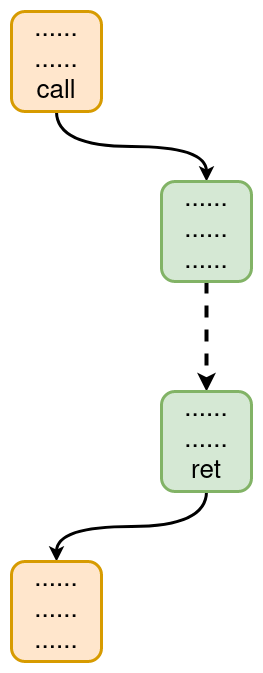
\includegraphics[width=.4\linewidth]{img/CallRetBefore.png}
		\caption{Original CFG}
	\end{subfigure}%
	\begin{subfigure}{.5\textwidth}
		\centering 	
		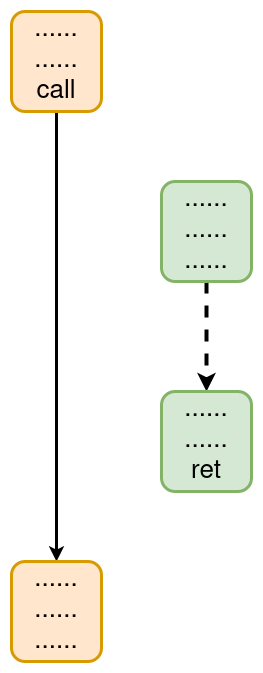
\includegraphics[width=.4\linewidth]{img/CallRetAfter.png}
		\caption{Transformed CFG}
	\end{subfigure}
	
	\caption{Transformation of the CFG around call/ret}
	\label{fig:callRet}
\end{figure}
 
\subsection{Finding the fetch}

\subsubsection{Basic Method}

The basic idea to find the fetch is to assume that all opcodes share the same basic block for the fetch, as in Figure \ref{fig:abstractVM:Centralized}.
Note that this is a somewhat restrictive assumption, albeit necessary for this method to work. Some VM implementations use a fetch block for each different opcode (see Figure \ref{fig:abstractVM:Decentralized}) : most notably CPython does so. This optimization ('computed-gotos') can thankfully be disabled when compiling CPython. In all my experiments I used this modified CPython version.
% todo : reference the CPython source file that implements computed gotos ?

\begin{figure}[htp]
	\centering
	\begin{subfigure}{.5\textwidth}
		\centering 	
		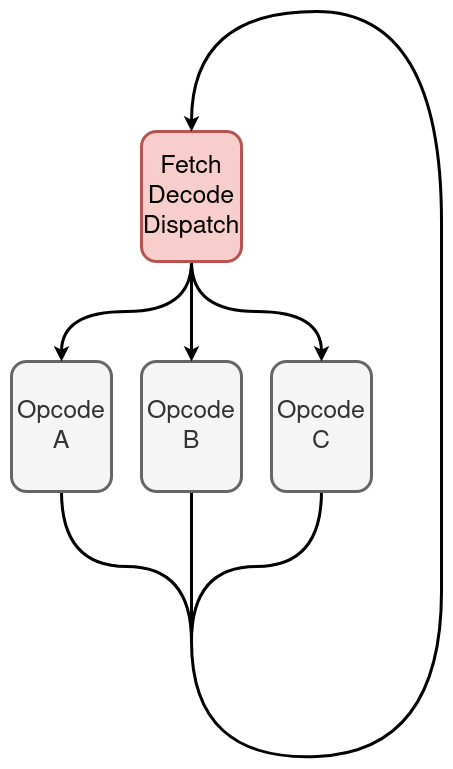
\includegraphics[width=.7\linewidth]{img/FetchCentralized.png}
		\caption{Centralized fetch}
		\label{fig:abstractVM:Centralized}
	\end{subfigure}%
	\begin{subfigure}{.5\textwidth}
		\centering 	
		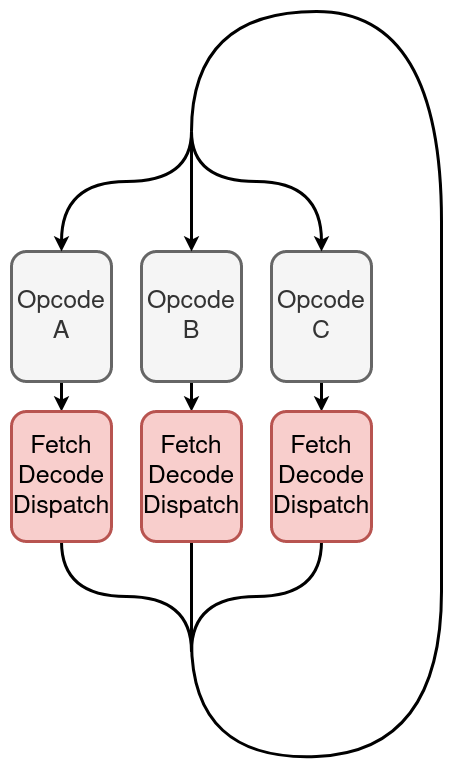
\includegraphics[width=.7\linewidth]{img/FetchDecentralized.png}
		\caption{Decentralized fetch ('computed-gotos')}
		\label{fig:abstractVM:Decentralized}
	\end{subfigure}
	\caption{Examples of VM control flow graphs}
	\label{fig:abstractVM}
\end{figure}

We thus build the CFG $\mathcal{C}$ and look for a basic block that :
\begin{itemize}
	\item is executed a large number of times (because it is shared between all opcodes).
	\item contains at least one instruction that reads a few bytes from memory (the fetch).
	\item has a large number of outgoing edges (the dispatch).
\end{itemize} 

Unfortunately, this method is too restrictive: the fetch, decode and dispatch aren't always in the same basic block in $\mathcal{C}$. There can be branches (e.g. to check for a termination condition, etc.) between the fetch and the dispatch, as shown in (ref to unfiltered cfg image). 

\subsubsection{Using the filtered CFG}

To handle this issue, we first filter out irrelevant detail from $\mathcal{C}$, and then hope that the fetch-decode-dispatch are in the same basic block in the new CFG $\mathcal{C}_{filtered}$. 

Given two parameters $exec\_blocks$ and $exec\_edges$, we build $\mathcal{C}_{filtered}$ as follows : 
\begin{itemize}
	\item For each block $B \in \mathcal{C}$, if $B$ is executed at least $exec\_blocks$ times, add $B$ to $\mathcal{C}_{filtered}$.
	\item For each edges $(E: B \rightarrow B') \in \mathcal{C}$, if $E$ is executed at least $exec\_edges$ times and both $B$ and $B'$ are executed at least $exec\_blocks$ times, add $E$ to $\mathcal{C}_{filtered}$.
\end{itemize}
We then apply a simple transformation on $\mathcal{C}_{filtered}$ to merge all blocks $B$ and $B'$ such that $next(B) = \{B'\}$ and $prev(B') = \{B\}$. During my experiments I had to tune the values of $exec\_blocks$ and $exec\_edges$, and found values around $1000$ to give satisfactory results. This method thus only works on Python programs that contain at least a few thousand opcodes.

The CFG $\mathcal{C}_{filtered}$ only retains the main structure of the graph, abstracting away the code paths rarely taken. However we might remove some or most of the opcode execution code from the graph (we only retain the opcodes executed a lot of times) (maybe image comparing filtered and unfiltered ?): $\mathcal{C}$ is a good place to look for the dispatch, and $\mathcal{C}_{filtered}$ is the place to look for the fetch-decode-dispatch basic block. 

We thus look for a basic block in $\mathcal{C}_{filtered}$ that :
\begin{itemize}
	\item is executed a large number of times.
	\item contains at least one instruction that reads a few bytes from memory (the fetch).
	\item contains at least one instruction that has a large number of outgoing edges in $\mathcal{C}$.
\end{itemize}

Once we have found the fetch, it is easy to find the bytecode : we simply get the value read by the fetch. We can also divide the trace into chunks corresponding to each bytecode, and remove the irrelevant parts of the VM trace (initialization and finalization code) : we obtain a list of small traces for each bytecode.

\begin{figure}[htp]
	\centering
	\begin{subfigure}{.5\textwidth}
		\centering 	
		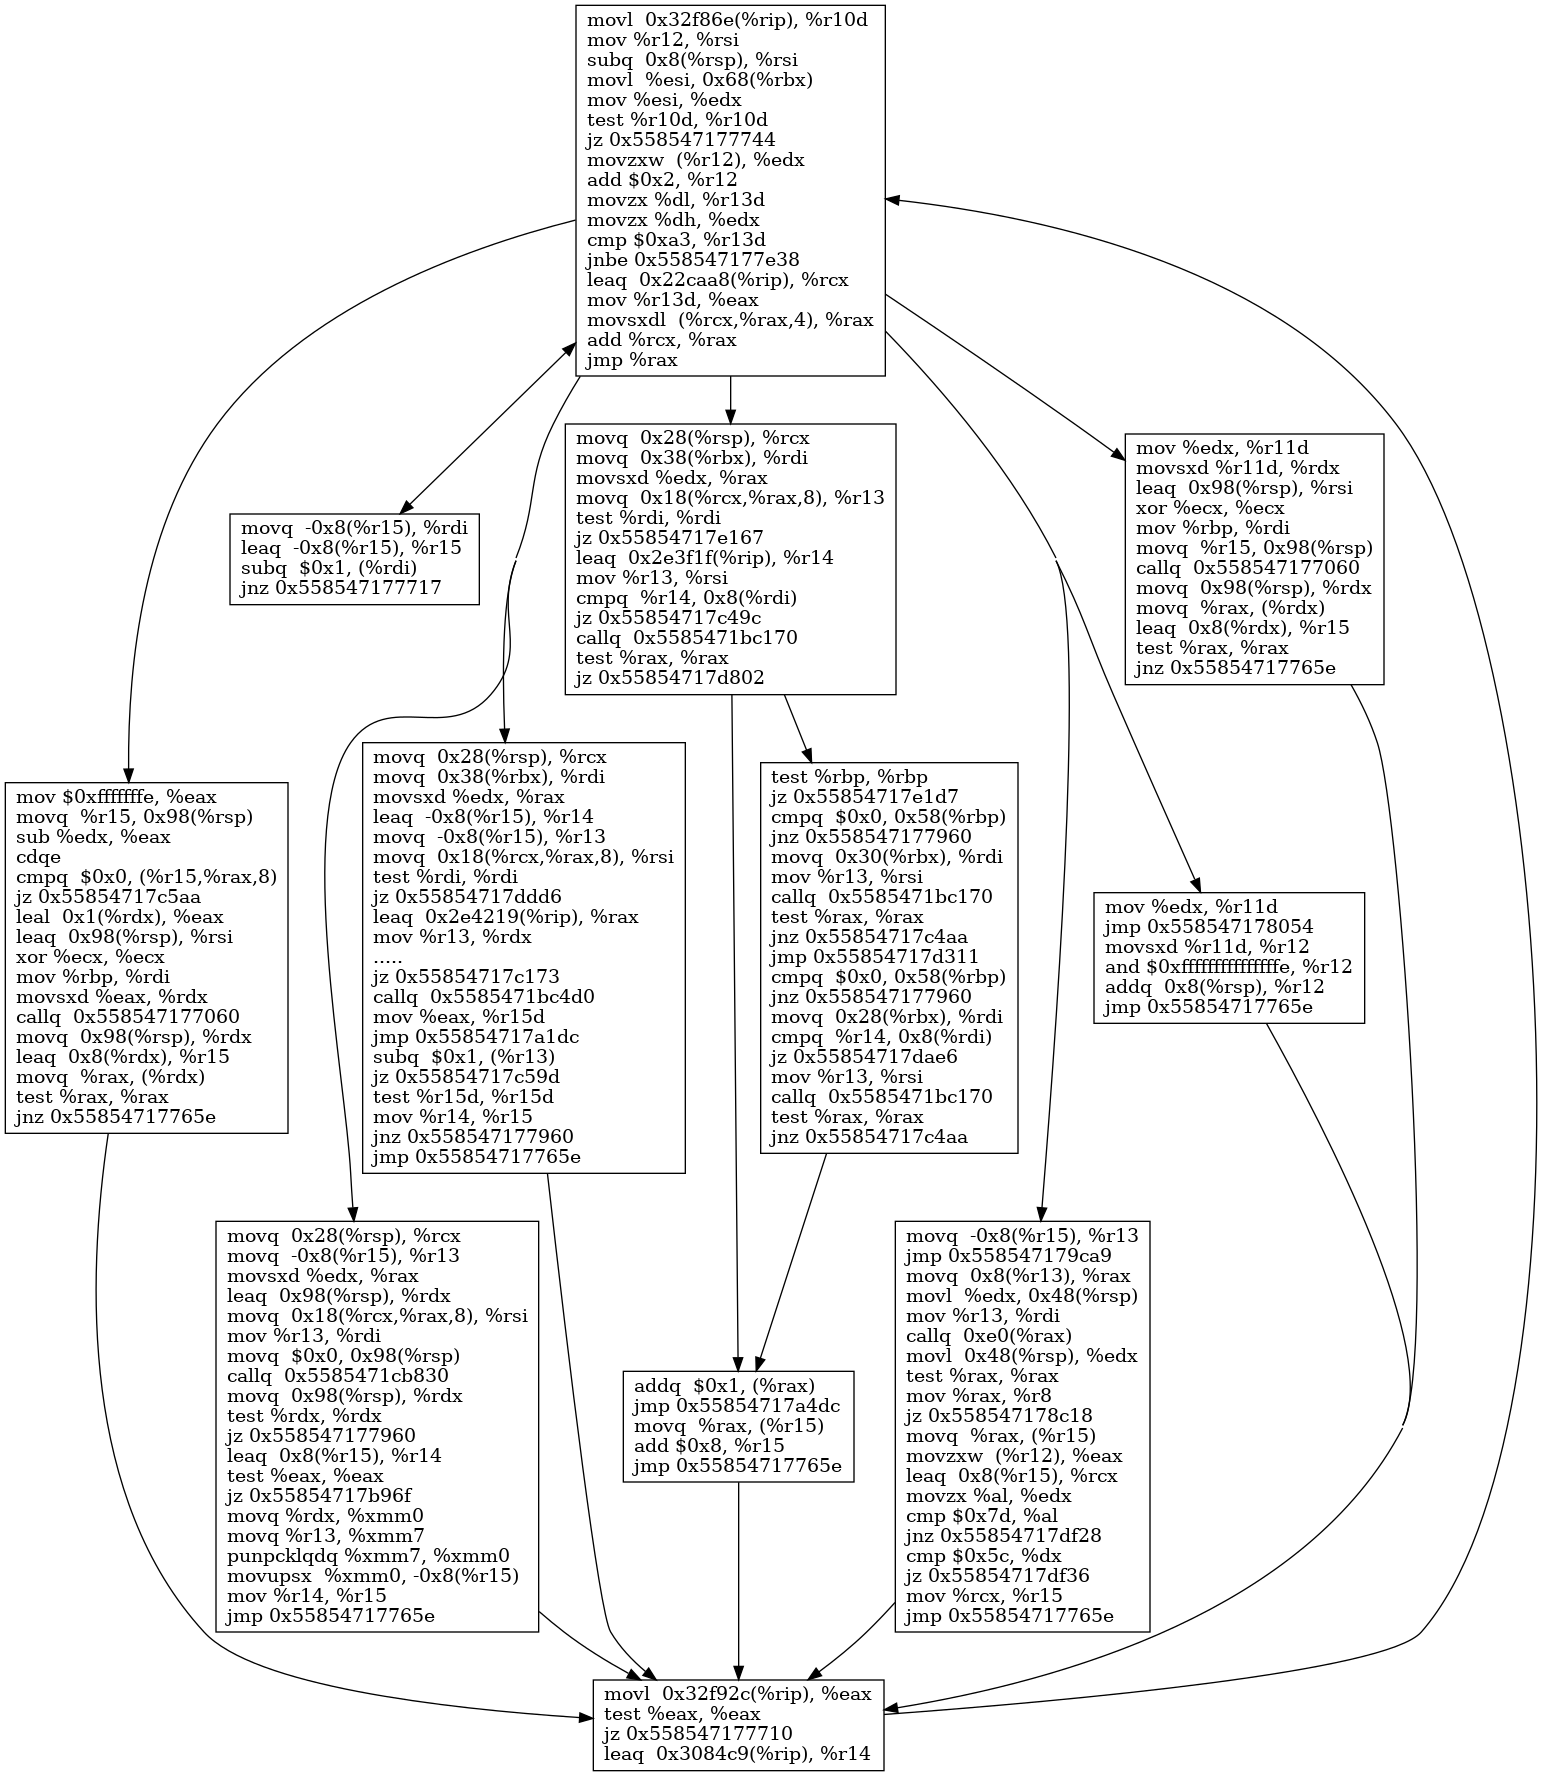
\includegraphics[width=.7\linewidth]{img/ConcreteVMFiltered.png}
		\caption{The relevant part of $\mathcal{C}_{filtered}$}
		\label{fig:concreteVM:Filtered}
	\end{subfigure}%
	\begin{subfigure}{.5\textwidth}
		\centering 	
		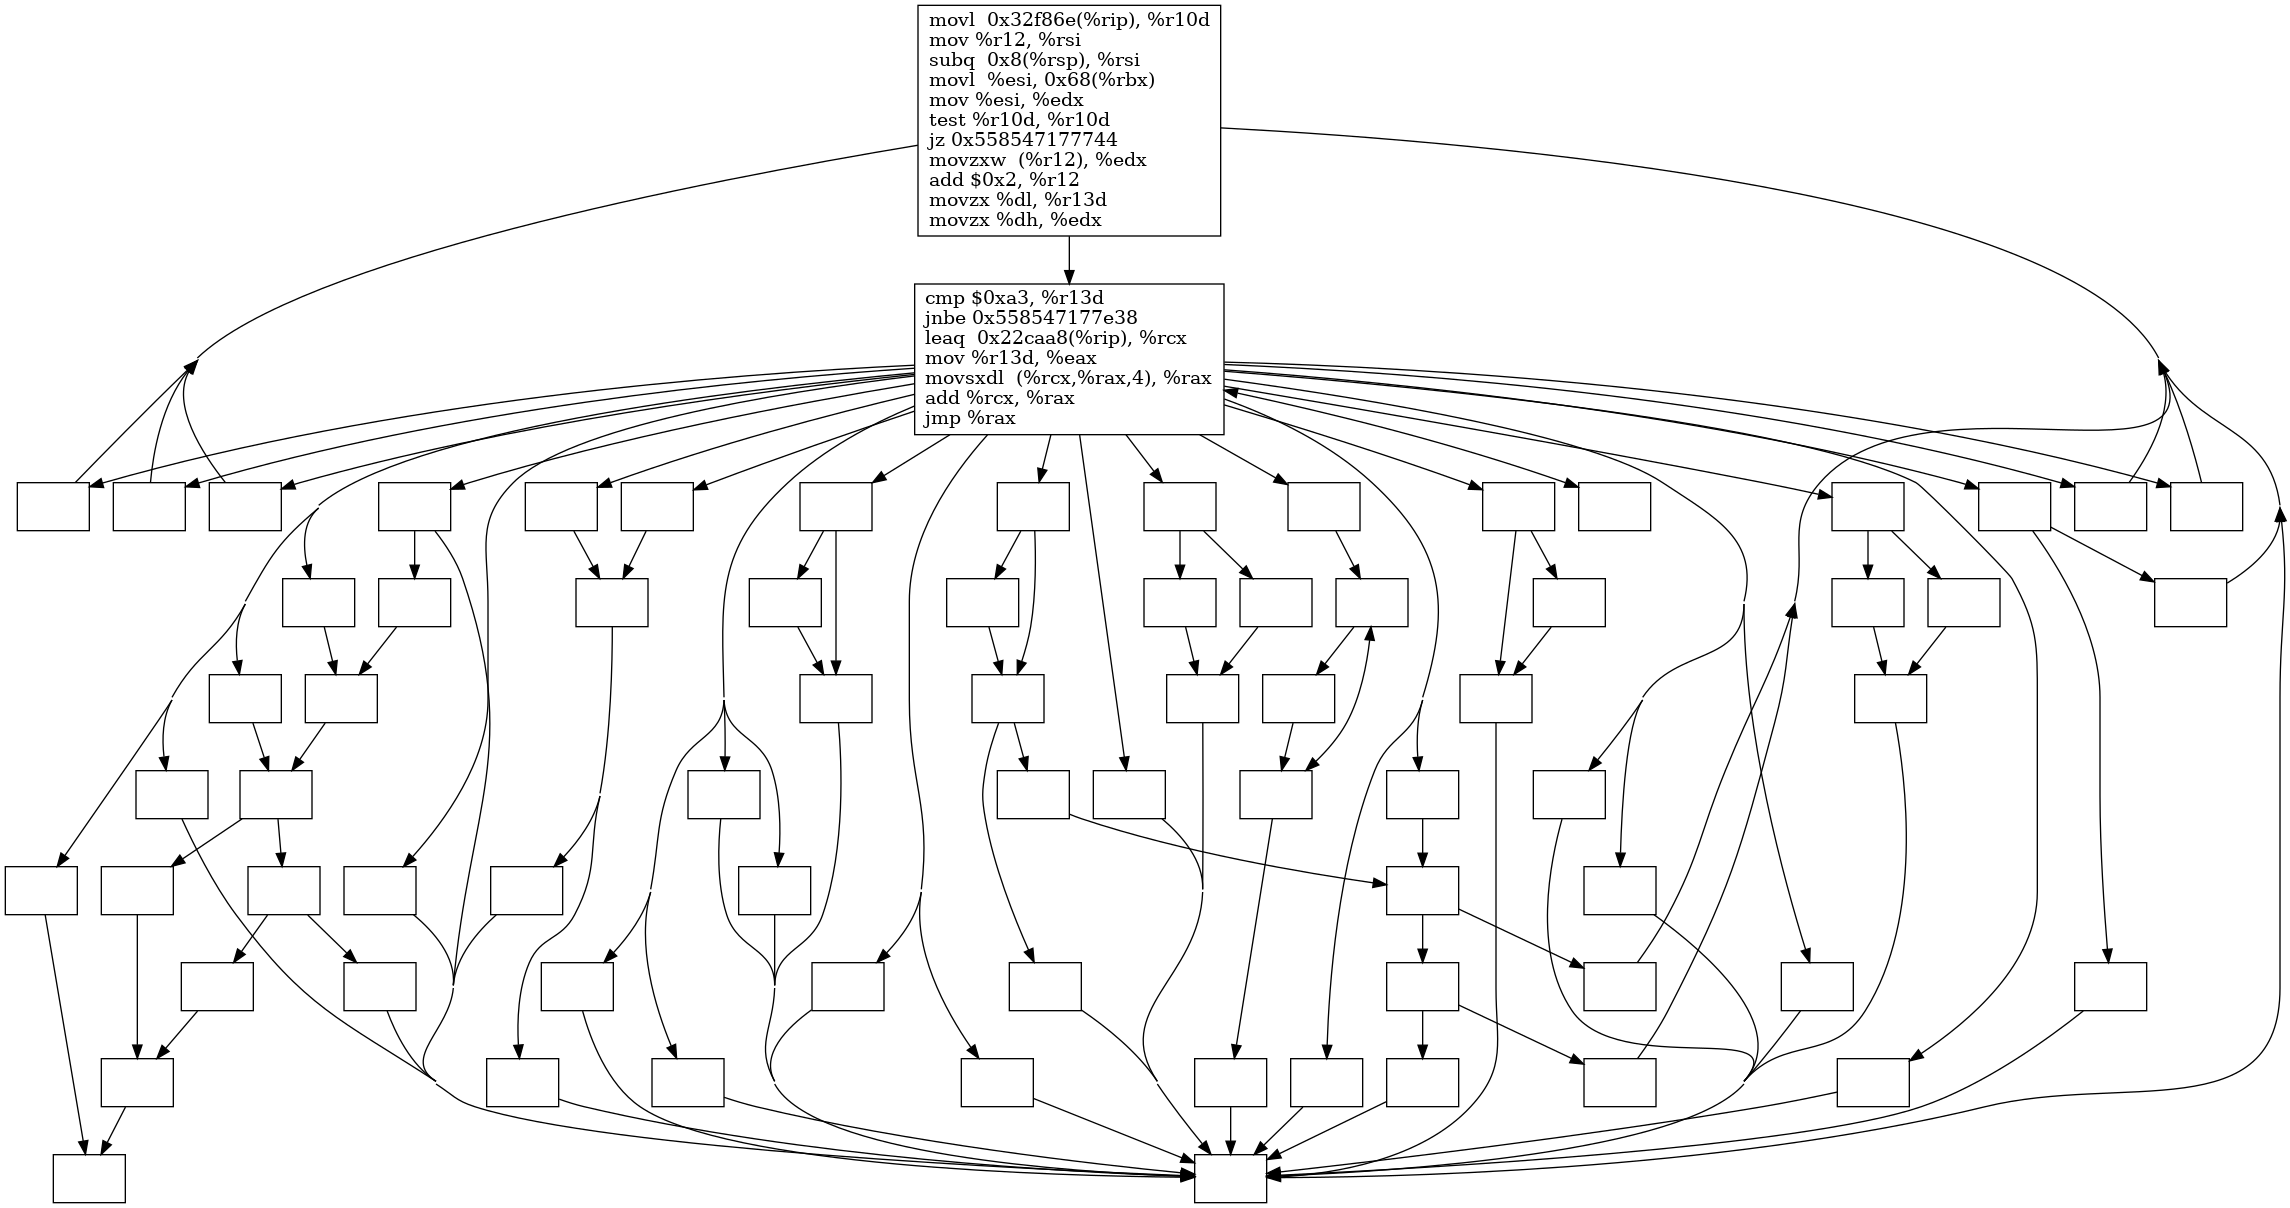
\includegraphics[width=.7\linewidth]{img/ConcreteVMOriginal.png}
		\caption{The relevant part of $\mathcal{C}$}
		\label{fig:concreteVM:Original}
	\end{subfigure}
	% todo : rephrase + add a reference to the python program (prog.py)
	\caption{VM control flow graphs for a trace using CPython}
	\label{fig:concreteVM}
\end{figure}


\section{Abstract VM model}

Before we can continue the analysis any further, we give ourselves an abstract VM model. While the previous section didn't assume much about the VM, this model follows more closely the Python VM.
\subsection{Definition}

We assume a stack-based VM, with no registers. It's internal state consists in :
\begin{itemize}
	\item a set of code blocks 
	\item a set of value stacks 
	\item a stack of frames.  
	\item pointers to the current frame ($fp$), the current bytecode ($ip$) and the top of the current value stack ($sp$)
\end{itemize}

A code block is a list of instructions. Each instruction is 2 bytes wide, the first byte being the opcode (example : ADD, POP, JMP) and the second byte being an argument. A code block contains all the code a given Python function can execute.

A value stack is a stack of Python values (objects). The contents of the stack are opaque to us. However all the values in the stack are contiguous in memory and of the same size.

Each frame corresponds to the execution of some Python function. A frame has its own code block and value stack.

The term "pointer" is intentionally vague : a pointer could be stored in a physical register or in a memory cell, it could contain the address of the object it points to or be an index into a list. During experiments I had to make additional assumptions about pointers, as will be explained in the following sections.

We will write $ptr \leftarrow f(ptr)$ where $f$ is any function and $ptr$ is $ip$, $sp$ or $fp$ to indicate that a given opcode changes the value of $ptr$ to $f(ptr)$.

\subsection{Finding pointers}

We assume the state of the VM is valid at the fetch (and at the dispatch). At other points in the execution trace, the registers and memory cells used to store the VM pointers may be used for different purposes. Our goal is then to find the most information we can about the VM state before each bytecode.

\subsubsection{Finding $ip$}

Our method for finding the fetch gives us the instruction(s) that read the bytecode, and thus the address of the bytecode in memory : this gives us the value of $ip$ before each opcode.

\subsubsection{Finding $fp$}

To find the frame pointers, we must make another assumption : that the C stack of the interpreter corresponds to the stack of the Python program it is running (remember we only look at the program state between bytecodes). Changes in $\%rsp$ should then give us the points at which the frame changes. Looking at registers that also change exactly and only at the same time as $\%rsp$ (and are also aligned on 8 bits) gives us additional frame pointers : pointers to some frame data (for instance, a C struct on the heap).

% todo : expand on this
Knowing the values of the frame pointers, we then tried to recognize the stack structure of frames, but some opcodes seem to operate on the stack of frame in non-standard ways : i.e. other than push or pop one, a even several, frame(s).

\subsubsection{Finding $sp$}

A first challenge is where to look for $sp$ : registers or memory ? It turns out it can be in both, depending on the interpreter (in a register for CPython, in memory for PyPy). Looking for $sp$ in registers is straightforward, as there are a very limited number of them. However memory is more complex : we can't scan through each memory cell. What we can hope for is that $sp$ is stored in a C struct pointed to by a frame pointer : $sp$ must be used very often, so requiring more than one pointer indirection to access it seems very inefficient. We thus look for $sp$ near addresses pointed to by frame pointers.  More precisely, we assume $sp$ will always be stored at $[fp + ofs]$ for $fp$ a frame pointer (whose value can change during the program execution) and $ofs$ a small constant offset (a multiple of 8).

To detect whether a location (register or memory cell) stores the value of $sp$, we take the list of values this location holds for each opcode. The basic idea is that many opcodes modify $sp$ in the same way : pop or push a few values. But we must be careful : we do not know whether $sp$ is stored as the address of the top stack cell, or as the index of the top stack cell, or something else. Depending on the case, a PUSH might increment $sp$ by $8$, $1$ or something else. The solution is to compute the alignment of $sp$, i.e. the largest power of $2$ that divides all the values in the list. We implement this idea as :
\begin{itemize}
	\item Compute the maximum consecutive number of times that $sp \leftarrow sp + k*align$ where $k$ is a small constant (e.g. $-2 \leq k \leq 2$). This number shouldn't change much with the size of the program (we check consecutive occurences) : we require it to be larger than a constant (e.g. $10$).
	\item Compute the maximum (not necessarily consecutive) number of times that $sp \leftarrow sp - align$, i.e. the number of POPs. This number should be proportional to the size of the program : we check it is larger than a percentage of the total opcode count (e.g. $10\%$).
\end{itemize}
The second test used is to distinguish between $sp$ and $ip$/$fp$: $ip$ and $fp$ might be stored in a similar way as $sp$, and pass the first test. 

\subsubsection{Code blocks}

We compute the code blocks by partitioning the bytecode instructions according to (transitive closure of) the following relation. Two bytecode instructions are in the same code block if :
\begin{itemize}
	\item They are executed in the same frame (i.e. there is no frame change between two of their executions). This is because all instructions executed inside a frame are in the same Python function.
	\item They are close in memory. This is because different code blocks are likely to be far apart in memory. % todo : why ?
\end{itemize}


\section{Opcode semantics}


\section{Experimental setup \& conclusion}


\end{document}


